\documentclass[12pt]{article}

\title{\vspace{-3em}PHYS 161a HW 2}
\author{Michael Cardiff}
\date{\today}

%% science symbols 
\usepackage{amsmath}
\usepackage{amssymb}
\usepackage{physics}
\usepackage{slashed}

%% general pretty stuff
\usepackage{bm}
\usepackage{enumitem}
\usepackage{float}
\usepackage{graphicx}
\usepackage[margin=1in]{geometry}
\usepackage[labelfont=bf]{caption}
\usepackage{tikz}

% figures
\graphicspath{ {./figs/} }

\newcommand{\fig}[3]
{
  \begin{figure}[H]
    \centering
    \includegraphics[width=#1cm]{#2}
    \caption{#3}
  \end{figure}
}

\newcommand{\figref}[4]
{
  \begin{figure}[H]
    \centering
    \includegraphics[width=#1cm]{#2}
    \caption{#3}
    \label{#4}
  \end{figure}
}

\newcommand*\circled[1]{\tikz[baseline=(char.base)]{
            \node[shape=circle,draw,inner sep=2pt] (char) {#1};}}
\renewcommand{\L}{\mathcal{L}}
\newcommand{\D}{\partial}
\newcommand{\munu}{{\mu\nu}}
\newcommand{\sla}[1]{\slashed{#1}}

\begin{document}
\maketitle
\section*{Problem 1}
\subsection*{Part 1}
This generalization theorem involves a rank 2 tensor instead of a vector, which is a rank 1 tensor. However, this is a fairly simple problem, we can see one index of the tensor is a vector. The transformation laws of a rank 2 tensor are:
\begin{align*}
  T_{AB}=T_{\alpha\beta}\pdv{x_\alpha}{x_A}\pdv{x_\beta}{x_B}
\end{align*}
This is most likely not right with index contractions and such. However, if we contract one index, that is, take a tensor dot product with a vector
\begin{align*}
  T_{AB}\dd{S}_A
\end{align*}
We are left with one index remaining, which means this is a vector quantity. For all values of $k=0...n$ we have the following:
\begin{gather*}
  \int\pdv{T_{i0}}{x_i}\dd{V}\\
  % \int\pdv{T_{i1}}{x_i}\dd{V}\\
  \vdots\\
  \int\pdv{T_{in}}{x_i}\dd{V}
\end{gather*}
Each of these individual quantities can be treated as an instance of the divergence theorem, with the partial with respect to $x_i$ being the gradient, and we can contract it with the $i$ in  $T_{ik}$. Which means we can replace the partial and $\dd{V}$ with a dot into $\dd{S}$, which in index notation would be $A_i\dd{S_i}$ for a vector $A$. Meaning we have:
\begin{gather*}
  \int_V\pdv{T_{i0}}{x_i}\dd{V}=\int_S T_{i0}\dd{S_i}\\
  % \int_V\pdv{T_{i1}}{x_i}\dd{V}=\int_S T_{i1}\dd{S_i}\\
  \vdots\\
  \int_V\pdv{T_{in}}{x_i}\dd{V}=\int_S T_{in}\dd{S_i}
\end{gather*}
We realize that we simply have $n$ independent divergence theorems, and since we want to write compactly, we can label it with an index $k$, therefore:
\begin{gather}
  \boxed{\int_V\pdv{T_{ik}}{x_i}\dd{V}=\int_S T_{ik}\dd{S_i}}
\end{gather}
\subsection*{Part 2}
First we need to move the divergence into the integral:
\begin{align*}
  \grad_{\vb{r}}\vdot\int\frac{\vb{A}(\vb{r}')}{\abs{\vb{r}-\vb{r}'}}\dd[3]{r'}=
  \int\grad_{\vb{r}}\vdot
  {\qty(\frac{\vb{A}(\vb{r}')}{\abs{\vb{r}-\vb{r}'}})}\dd[3]{r'}
\end{align*}
Note that $\vb{A}$'s argument is primed, and the divergence is not, so it is constant with respect to the divergence, and hence we can turn it into a gradient of the scalar function $1/\abs{\vb{r-r}'}$ times a constant vector. In essence, we need to use this identity:
\begin{align*}
  \div{(\psi\vb{A})}=\psi\div{\vb{A}}+\vb{A}\vdot\grad{\psi}
\end{align*}
However, we can immediately say $\div{\vb{A}=0}$ here because $A$ is not a function of the divergence's coordinates:
\begin{align*}
  \grad_{\vb{r}}\vdot\qty(\frac{\vb{A}(\vb{r}')}{\abs{\vb{r-r}'}})=
  \qty(\grad_{\vb{r}}{\frac1{\abs{\vb{r-r}'}}})\vdot\vb{A}(\vb{r}')
\end{align*}
However, now we need to make use of the following identity, for a function $f(x-x')$
\begin{align*}
  \pdv{f(x-x')}{x'}=-\pdv{f(x-x')}{x}
\end{align*}
Then we can move the gradient from a $r\to r'$ using the following:
\begin{align*}
  \grad_{\vb{r}}=-\grad_{\vb{r}'}
\end{align*}
Which turns our quantity into:
\begin{align*}
  \qty(\grad_{\vb{r}}{\frac1{\abs{\vb{r-r}'}}})\vdot\vb{A}(\vb{r}')=
  -\qty(\grad_{\vb{r}'}{\frac1{\abs{\vb{r-r}'}}})\vdot\vb{A}(\vb{r}')
\end{align*}
Using the same vector calculus identity as before but with a no longer constant $\vb{A}$:
\begin{align*}
  -(\grad{\psi})\vdot\vb{A}=-\div{(\psi\vb{A})}+\psi\div\vb{A}
\end{align*}
Now that we have the same coordinates on the divergence as we have in the field $\vb{A}$, we can use our first condition, that $\div{\vb{A}}=0$, leaving us with:
\begin{align*}
  -\int_V\grad_{\vb{r}'}\vdot\qty(\frac{\vb{A}(\vb{r}')}{\abs{\vb{r-r}'}})
  \dd[3]{r'}
\end{align*}
We can then use the divergence theorem:
\begin{align*}
  -\int_V\grad_{\vb{r}'}\vdot\qty(\frac{\vb{A}(\vb{r}')}{\abs{\vb{r-r}'}})
  \dd[3]{r'}=\oint_{\D V}\qty(\frac{\vb{A}(\vb{r}')}{\abs{\vb{r-r}'}})
  \vdot\dd{\vb{S}}
\end{align*}
Note that the form of $\dd{\vb{S}}=\vu{n}\dd{S}$, and since $\vb{A}\vdot\vu{n}=A_n=0$ is our other condition, we can conclude that the integral is in fact $0$:
\begin{align}
  \boxed{
    \grad_{\vb{r}}\vdot\int
    \frac{\vb{A}(\vb{r}')}{\abs{\vb{r}-\vb{r}'}}\dd[3]{r'}=0
  }
\end{align}
\newpage
\section*{Problem 2}
\subsection*{Part 1}
The Fourier series for a function in terms of $e^{int}$ is given by:
\begin{align*}
  g(t)=\sum_{n=-\infty}^{\infty}A_n\exp(int)
\end{align*}
With the coefficient being:
\begin{align*}
  A_n=\frac{1}{2\pi}\int_0^{2\pi}g(t)e^{-int}\dd{t}
\end{align*}
Plug in $g(t)$:
\begin{align*}
  A_n&=\frac{1}{2\pi}\int_0^{2\pi}
  \qty(\frac{\pi^2}{6}-\frac12(t-\pi)^2)e^{-int}\dd{t}\\
  &=\frac\pi{12}\int_0^{2\pi}e^{-int}\dd{t}
  -\frac{1}{4\pi}\int_0^{2\pi}(t-\pi)^2e^{-int}\dd{t}\\
  &=\frac{\pi}{12}\circled{1}-\frac{1}{4\pi}\circled{2}
\end{align*}
Evaluate each integral:
\begin{align*}
  \circled{1}&=\int_0^{2\pi}e^{-int}\dd{t}\\
  &=\eval{\frac{i}{n}e^{-int}}_{0}^{2\pi}\\
  &=\frac{i}{n}\qty(e^{-2n\pi i}-1)
\end{align*}
Using Euler's identity gives that the exponential value is $1$ so this integral does not contribute:
\begin{align*}
  \circled{1}=0
\end{align*}
The next integral is:
\begin{align*}
  \circled{2}&=\int_0^{2\pi}(t-\pi)^2e^{-int}\dd{t}\\
  x&=t-\pi \quad \dd{x}=\dd{t}\\
  &=\int_{-\pi}^{\pi}x^2e^{-in(x+\pi)}\dd{x}\\
  &=\int_{-\pi}^\pi x^2e^{-inx}e^{-i\pi n}\dd{x}\\
  &=(-1)^n\int_{-\pi}^{\pi}x^2e^{-inx}\dd{x}
\end{align*}
Using integration by parts we can reduce this integral:
\begin{align*}
  \int_{-\pi}^{\pi}x^2e^{-inx}\dd{x}&=\eval{\frac{ix^2e^{-inx}}{n}}_{-\pi}^\pi
  -\frac{2i}{n}\int_{-\pi}^\pi xe^{-inx}\dd{x}\\
  \int_{-\pi}^\pi xe^{-inx}\dd{x}&=\eval{\frac{ixe^{-inx}}{n}}_{-\pi}^\pi
  -\frac{i}{n}\int_{-\pi}^\pi e^{-inx}\dd{x}\\
  -\frac{i}{n}\int_{-\pi}^\pi e^{-inx}\dd{x}&=
  \eval{-\frac{e^{-inx}}{n^2}}_{-\pi}^\pi
\end{align*}
The total antiderivative is then:
\begin{align*}
  \eval{e^{-inx}\qty(\frac{ix^2}{n}+\frac{2x}{n^2}-\frac{2i}{n^3})}_{-\pi}^\pi
\end{align*}
Evaluate at the bounds:
\begin{align*}
  \eval{e^{-inx}\qty(\frac{ix^2}{n}+\frac{2x}{n^2}-\frac{2i}{n^3})}_{-\pi}^\pi
  =e^{in\pi}\qty(\frac{2i}{n^3}+\frac{2\pi}{n^2}-\frac{i\pi^2}{n})
  +e^{-in\pi}\qty(-\frac{2i}{n^3}+\frac{2\pi}{n^2}-\frac{i\pi^2}{n})
\end{align*}
Note how the terms with odd powers of $n$ in the denominator have opposite signs, these will create the $\sin$ function when combined, and $\sin(n\pi)$ is $0$, where the term with an even power of $n$ in the denominator makes a cosine, and since $\cos(n\pi)=(-1)^n$ we get:
\begin{align*}
  \circled{2}=(-1)^n(-1)^n\frac{4\pi}{n^2}=\frac{4\pi}{n^2}
\end{align*}
Now back to our original combination:
\begin{align*}
  \frac\pi{12}\circled{1}-\frac1{4\pi}\circled{2}=-\frac{1}{n^2}
\end{align*}
Hence the Fourier series is:
\begin{align}
  \boxed{
    g(t)=-\sum_{n=-\infty,\neq0}^\infty\frac{e^{int}}{n^2}
  }
\end{align}
\subsection*{Part 2}
In terms of its fourier series, the first and second derivatives are:
\begin{equation}
  \boxed{
    \begin{aligned}
      g'(t)&=-i\sum_{n=-\infty,\neq0}^\infty\frac{e^{int}}{n}\\
      g''(t)&=\sum_{n=-\infty,\neq0}^\infty e^{int}
    \end{aligned}
  }
\end{equation}
Note that there is no disncontinuity in $g$, so we only need the classical derivative. However the derivative $g'$ is discontinuous, so we do in fact need the sum of $\delta$ functions, note the height of the discontinuity is $2\pi$:
\begin{equation}
  \boxed{
    \begin{aligned}
      g'(t)&=-(t-\pi)\\
      g''(t)&=-1+2\pi\sum_{k=-\infty}^\infty\delta(t-2k\pi)
    \end{aligned}
  }
\end{equation}
The following is two periods of each function:
\begin{figure}[H]
  \centering
  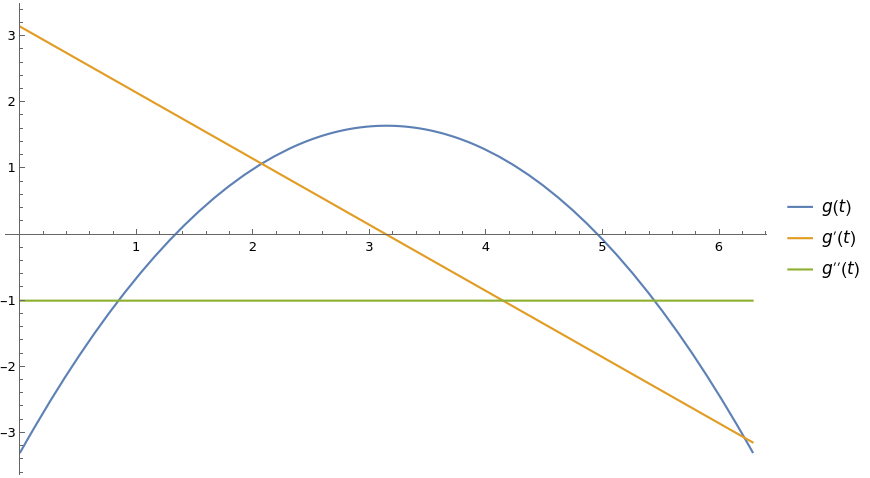
\includegraphics[width=10cm]{fourierplot.png}
  \caption{One Period of $g(t), g'(t)$, and $g''(t)$}
  \label{fig:1}
\end{figure}
\subsection*{Part 3}
First we need to see if this sum will converge in the distributional sense. If we can identify a function $h(t)$ such that $f(t)$ is one of the derivatives of that function, and that function converges classically, then that function $h(t)$ will converge distributionally, so its derivatives will converge distributionally as well. We can recognize one such function is the Fourier series of $g(t)$. Mainly that:
\begin{align*}
  \dv[2]{t}\qty(-\sum_{n=-\infty,\neq0}^\infty\frac{e^{int}}{n^2})=\sum e^{int}
\end{align*}
It will then converge in the distributional sense. The value can be found by applying to a test function:
\begin{align}
  \ip{\sum_{-\infty}^\infty e^{int}}{\phi}
  =\ip{-1+2\pi\sum_{k=-\infty}^{\infty}\delta(t-2k\pi)}{\phi}
\end{align}
Thus, we find:
\begin{align*}
  \ip{-1+2\pi\sum_{k=-\infty}^{\infty}\delta(t-2k\pi)}{\phi}
  =-\ip{\mathbb{I}}{\phi}+2\pi\sum_{k=-\infty}^{\infty}\phi(2k\pi)
\end{align*}
The sum was found to be:
\begin{align*}
  2\pi\sum_{-\infty}^\infty\phi(2k\pi)=\ip{\mathbb{I}}{\phi}+2\ip{\cos(nt)}{\phi}
\end{align*}
Hence:
\begin{align}
  \boxed{
    \ip{\sum_{-\infty}^\infty e^{int}}{\phi}=2\sum_{n=0}^\infty\ip{\cos(nt)}{\phi}
  }
\end{align}
I am giving up at this point
\newpage
\section*{Problem 3}
\subsection*{Part 1}
Since $\sin$ is a normally defined function, and $\phi$ is a test function, we can realistically write:
\begin{align*}
  \ip{\sin(at)\delta^{(1)}}{\phi(t)}=\ip{\delta^{(1)}}{\sin(at)\phi(t)}
\end{align*}
Since $\phi(t)$ has compact support, so will $\sin(at)\phi(t)$, thus we can use identities for distributions on this, namely that the derivative is given by:
\begin{align*}
  \ip{\delta^{(1)}}{\sin(at)\phi(t)}=-\ip{\delta}{(\sin(at)\phi(t))'}
\end{align*}
From which we can compute a classical derivative:
\begin{align*}
  (\sin(at)\phi(t))'=a\cos(at)\phi(t)+\sin(at)\phi'(t)
\end{align*}
Then we can use the definition of the delta:
\begin{align*}
  \ip{\delta}{\chi(t)}=\chi(0)
\end{align*}
With the definition of $\chi$ as the derivative above, we get:
\begin{align*}
  -\ip{\delta}{a\cos(at)\phi(t)+\sin(at)\phi'(t)}=
  -a\cos(0)\phi(0)-\sin(0)\phi'(0)=-a\phi(0)
\end{align*}
Hence:
\begin{align*}
  \ip{\sin(at)\delta^{(1)}}{\phi(t)}=-a\phi(0)=\ip{-a\delta}{\phi}
\end{align*}
Thus we can conclude:
\begin{align}
  \boxed{\sin(at)\delta^{(1)}=-a\delta}
\end{align}
\subsection*{Part 2}
This requires we prove the product rule holds for a smooth function $g$ times a distribution $T$. Start with the definition of the distributional derivative:
\begin{align*}
  \ip{(gT)'}{\phi}=-\ip{gT}{\phi'}
\end{align*}
We can move $g$ onto the test function by the definition of a distribution by a smooth function:
\begin{align*}
  -\ip{gT}{\phi'}=-\ip{T}{g\phi'}
\end{align*}
These are now two classical functions, so the regular product rule applies:
\begin{align*}
  g\phi'=(g\phi)'-g'\phi
\end{align*}
Plugging this in:
\begin{align*}
  -\ip{T}{g\phi'}=-\ip{T}{(g\phi)'-g'\phi}
\end{align*}
Distributions are linear functionals:
\begin{align*}
  -\ip{T}{(g\phi)'-g'\phi}=-\qty(\ip{T}{(g\phi)'}-\ip{T}{g'\phi})
\end{align*}
We can then use the definition of the distributional derivative the other way now:
\begin{align*}
  -\ip{T}{(g\phi)'}+\ip{T}{g'\phi}=\ip{T'}{g\phi}+\ip{T}{g'\phi}
\end{align*}
Using the property of multiplying by a smooth function again in the other direction yields the distributional product rule:
\begin{align*}
  \ip{T'}{g\phi}+\ip{T}{g'\phi}=\ip{gT'}{\phi}+\ip{g'T}{\phi}
\end{align*}
Using linearity one last time is the explicit rule:
\begin{align*}
  \boxed{\ip{(gT)'}{\phi}=\ip{(gT'+g'T)}{\phi}}
\end{align*}
Thus we can apply it here:
\begin{align*}
  \dv[2]{t}\qty(H(t)\sin(at))&=\dv{t}\qty(a\cos(at)H(t)+\delta(t)\sin(at))\\
  &=-a^2H(t)\sin(at)+2a\cos(at)\delta(t)+\sin(at)\delta^{(1)}(t)
\end{align*}
Using our result for the derivative of the $\delta$ times sine in the previous part, we can write a since form:
\begin{align}
  \boxed{
    \dv[2]{t}\qty(H(t)\sin(at))=-a^2\sin(at)H(t)+(2\cos(at)-1)a\delta(t)
  }
\end{align}
\newpage
\section*{Problem 4}
Using Gauss's Law, we have that the charge density and the electric field are related by:
\begin{align*}
  \div{\vb{E}}=\frac{\rho}{\varepsilon_0}
\end{align*}
The spherical coordinates divergence is given by:
\begin{align*}
  \div{\vb{A}}=\frac{1}{r^2}\pdv{(r^2\vb{A}\vdot\vu{r})}{r}
  +\frac1{r\sin\theta}\pdv{\theta}(\vb{A}\vdot\bm{\hat\theta}\sin\theta)
  +\frac1{r\sin\theta}\pdv{\vb{A}\vdot\bm{\hat\phi}}{\phi}
\end{align*}
The only non-zero dot product would be $\vb{E}\vdot\vu{r}$:
\begin{align*}
  \div{\vb{E}}&=\frac1{r^2}\pdv{r}\qty(r^2E_0H(a-r))\\
  &=\frac1{r^2}\qty(E_0r\qty(2H(a-r)-rH'(a-r)))\\
  &=\frac{E_0}{r}\qty(2H(a-r)-rH'(a-r))
\end{align*}
If we work in a distributional sense, we know the derivative of the Heaviside function $H$ is a $\delta$:
\begin{align*}
  \div{\vb{E}}&=\frac{E_0}{r}\qty(2H(a-r)-r\delta(a-r))
\end{align*}
Multiplying by $\varepsilon_0$ gives the charge density:
\begin{align}
  \boxed{
    \rho=\varepsilon_0\frac{E_0}{r}\qty(2H(a-r)-r\delta(a-r))
  }
\end{align}
We can use the integral form of Gauss's law to get the total charge:
\begin{align*}
  Q=\varepsilon_0\oint E_0H(a-r)\vu{r}\vdot\dd{\vb{S}}
\end{align*}
The differential surface element at some $r$ is:
\begin{align*}
  \vu{r}\vdot\dd{\vb{S}}=r^2\sin\theta\dd{\theta}\dd{\phi}
\end{align*}
Integrating:
\begin{align*}
  Q&=\varepsilon_0E_0\int_0^\pi\int_0^{2\pi}H(a-r)
  r^2\sin\theta\dd{\theta}\dd{\phi}\\
  &=\varepsilon_0E_0r^2H(a-r)\int\dd{\Omega}\\
  &=4\pi\varepsilon_0r^2E_0H(a-r)
\end{align*}
The charge is:
\begin{align}
  \boxed{
    Q=4\pi\varepsilon_0r^2E_0H(a-r)
  }
\end{align}
Now the potential, which can be calculated by:
\begin{align*}
  \varphi(r)=-\int_{r_0}^r\vb{E}\vdot\dd{\bm{\ell}}
\end{align*}
Arbitrarily set $r_0=0$, and $r=r'$ to avoid confusion. The differential line element in spherical coordinates is:
\begin{align*}
  \dd{\bm{\ell}}=\vu{r}\dd{r}
  +\hat{\bm{\phi}}r\dd{\phi}
  +\hat{\bm{\theta}}r\sin\theta\dd{\theta}
\end{align*}
Therefore the only got that counts is the $\vu{r}$:
\begin{align*}
  \varphi(r')=-\int_0^{r'}E_0H(a-r)\dd{r}
\end{align*}
Then if $r'<a$ we can directly integrate:
\begin{align*}
  \varphi(r')_{r'<a}=-E_0r'
\end{align*}
If $r'>a$ then we have:
\begin{align*}
  \varphi(r')&=-\int_0^{r'}E_0H(a-r)\dd{r}\\
  &=-\int_0^aE_0H(a-r)\dd{r}-\int_a^{r'}E_0H(a-r)\dd{r}
\end{align*}
The second integral is $0$ as the argument of the heaviside function will be $0$ that entire region, the other is the same as before just evaluated at $a$:
\begin{equation}
  \boxed{
    \varphi(r)=
    \begin{cases}
      -E_0r & r<a \\
      -E_0a & r\geq a
    \end{cases}
  }
\end{equation}
\newpage
\section*{Problem 5}
We can immediately move the laplacian over to the test function $\phi$:
\begin{align*}
  \ip{\laplacian{\ln(r)}}{\phi}=\ip{\ln(r)}{\laplacian{\phi}}
\end{align*}
There is a discontinuity at $r=0$ so we can write:
\begin{align*}
  \ip{\ln(r)}{\laplacian{\phi}}=\lim_{\epsilon\to0}
  \int_{\abs{r}>\epsilon}\ln(r)\laplacian{\phi}\dd{r}
\end{align*}
We want to make use of Green's Identities:
\begin{align*}
  \int\div{\vb{F}}\dd[2]{r}=\oint\vb{F}\vdot\vu{n}\dd{\ell}
\end{align*}
Note our volume is now an area and the surface is now a curve.
We want to end up with something of the form:
\begin{align*}
  \int\qty(\phi\laplacian{\psi}-\psi\laplacian\phi)\dd[2]{r}=
  \int\qty(\phi\grad{\psi}-\psi\grad{\phi})\vdot\dd{\vb{\ell}}
\end{align*}
We then take $\psi=\ln(r)$ and $\laplacian{\psi}=0$:
\begin{align*}
  \int\ln(r)\laplacian{\phi}\dd[2]{r}=\int(\ln(r)\grad\phi-\phi\grad{\ln(r)})
  \vdot\vu{n}\dd{\ell}
\end{align*}
We realize that $\vu{n}\vdot\gradient=-\pdv{r}$ since we are using polar coordinates and our curve is oriented opposite to the normal.
\begin{align*}
  \int(\ln(r)\grad\phi-\phi\grad{\ln(r)})\vdot\vu{n}\dd{\ell}=
  \int\qty(-\ln(\epsilon)\pdv{\phi}{r}+\phi\frac{1}{r})
  r\dd{\varphi}
\end{align*}
The logic follows exactly the same as when we did the laplacian of $1/r$ in class:
\begin{align*}
  \ip{\laplacian{\ln(r)}}{\phi}=\ip{2\pi\delta}{\phi}
\end{align*}
Hence:
\begin{align}
  \boxed{
    \laplacian{\ln(r)}=2\pi\delta(r)
  }
\end{align}
\end{document}